\begin{center}
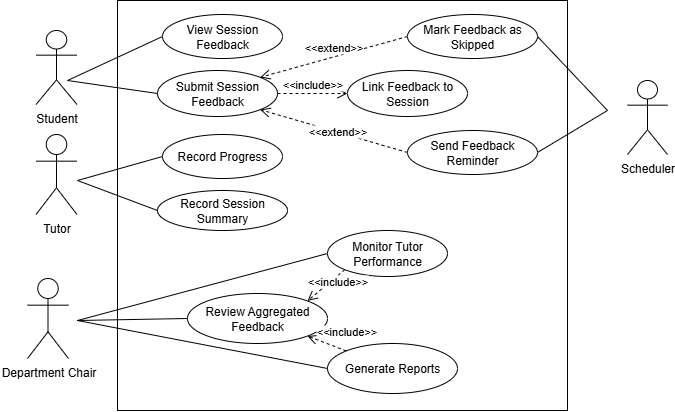
\includegraphics[width=0.9\linewidth]{images/UC-04.png}
\end{center}

\begin{center}
\textbf{Figure 5:}  Submit Session Feedback
\end{center}


\begin{table}[h!]
\centering
\begin{tabular}{|p{3cm}|p{11cm}|}
\hline
\textbf{Use-case ID} & UC-04 \\
\hline
\textbf{Use-case name} & Submit Session Feedback \\
\hline
\textbf{Use-case overview} & To allow a student to submit structured feedback after a tutoring session. The feedback is linked to the session and stored for later evaluation and reporting. \\
\hline
\textbf{Actors} & Student (primary), Scheduler (secondary, for reminders) \\
\hline
\textbf{Preconditions} & 
1. A tutoring session has been completed. \newline
2. The system is running and accessible. \newline
3. Student is authenticated in the system. \\
\hline
\textbf{Trigger} & The student clicks the ``Submit Feedback'' option after the session is completed. \\
\hline
\textbf{Steps} & 
1. System displays a feedback form linked to the completed session. \newline
2. Student fills in and submits the structured feedback. \newline
3. System validates the input and saves the feedback in the database. \newline
4. System links the feedback to the corresponding session. \newline
5. If no feedback is submitted within the allowed time, the Scheduler triggers reminders. \newline
6. If the deadline passes without submission, the system marks the feedback as ``Skipped.'' \\
\hline
\textbf{Postconditions} & 
1. Feedback is stored in the database and linked to the correct session. \newline
2. If skipped, the system records a ``Feedback Skipped'' status for that session. \newline
3. Data is available for tutors and department chairs in aggregated reports. \\
\hline
\textbf{Alternative Flows} & 
1. Multiple Session Feedback → If multiple sessions are pending, the system displays a list and allows the student to submit feedback sequentially. \newline
2. Draft Save → The student may save incomplete feedback as a draft and return later within the allowed timeframe. \newline
3. Feedback Revision → Within 24h, the student may edit and resubmit feedback; the updated version replaces the original record. \\
\hline
\textbf{Exception Flow} & 
1. If the student loses connection before submission, the system prompts the student to retry. \newline
2. If the session record is missing or corrupted, the system logs an error and notifies the coordinator. \\
\hline
\end{tabular}
\caption{Use Case UC-04: Submit Session Feedback}
\end{table}
